\documentclass[12pt]{article}

%
\usepackage{graphicx,amsmath}
%%%%%%%%%%%%%%%%%%%%%%%%%%%%%%%%%%%%%%%%
\usepackage{txfonts}
%%%%%%%%%%%%%%%%%%%%%%%%%%%%%%%%%%%%%%%%
\usepackage{hyperref}
% To add links in your PDF file, use the package "hyperref"
% with options according to your LaTeX or PDFLaTeX drivers.
%
\usepackage[english]{babel}


\oddsidemargin = -20pt
\topmargin = -50pt
\headheight = 12pt
\headsep = 25pt
\textheight = 700pt
\textwidth = 500pt
\marginparsep = 10pt
\marginparwidth = 35pt
\footskip = 30pt
\marginparpush = 7pt
\hoffset = 0pt
\voffset = 0pt
\paperwidth = 597pt
\paperheight = 845pt


%package not to center caption
\usepackage[labelfont=bf]{caption}
\usepackage{multicol}
\setlength{\columnsep}{20pt}

\begin{document} 


\begin{figure}
\centering
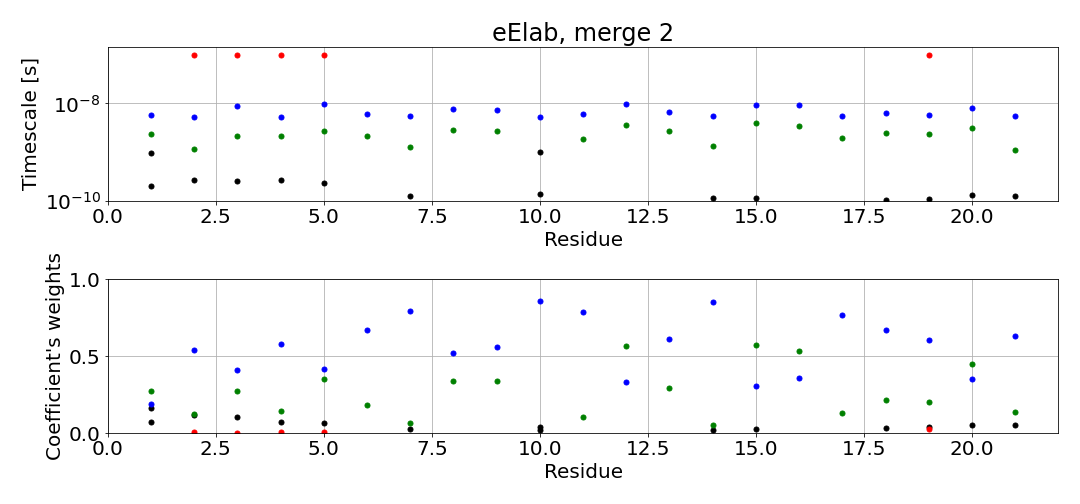
\includegraphics[width=0.5\textwidth]{eElab_2_slow.png}
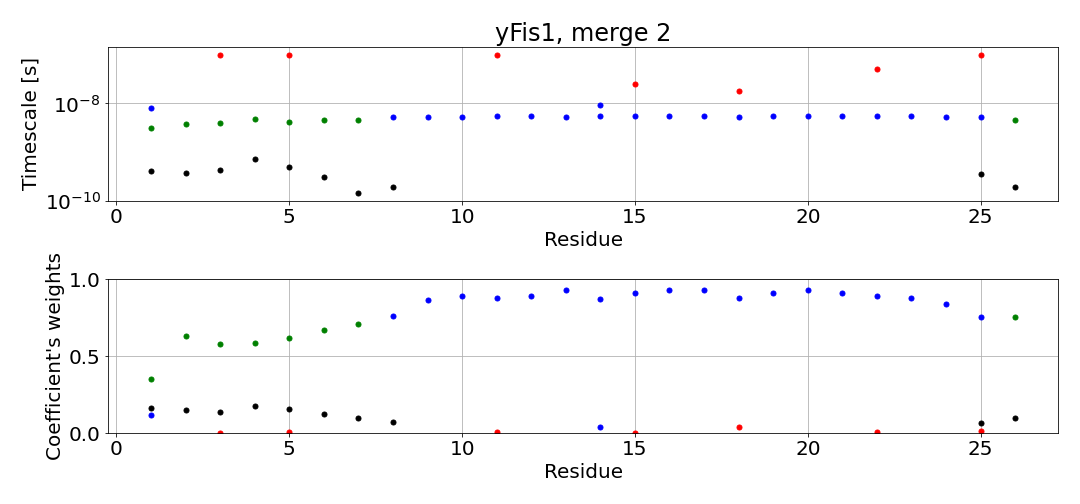
\includegraphics[width=0.5\textwidth]{yFis1_2_slow.png}
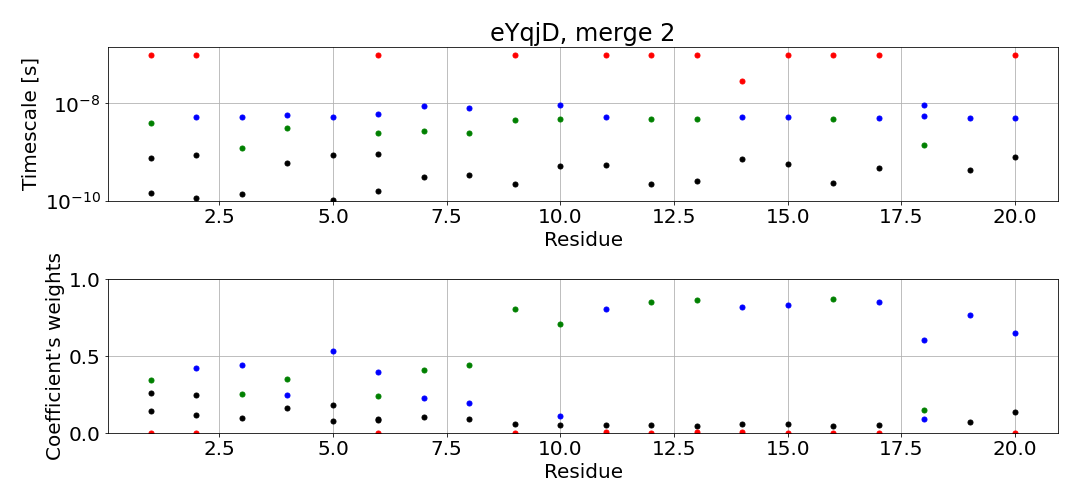
\includegraphics[width=0.5\textwidth]{eYqjD_2_slow.png}
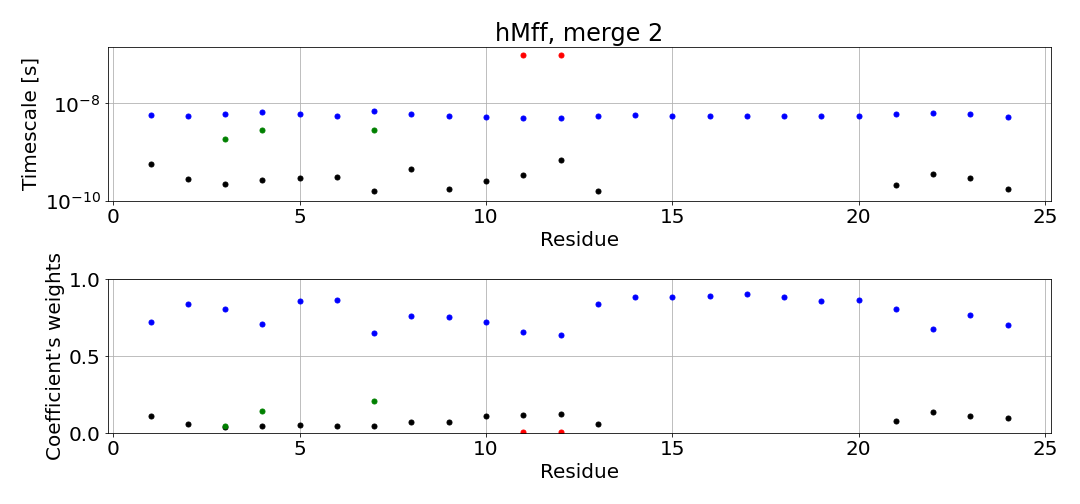
\includegraphics[width=0.5\textwidth]{hMff_2_slow.png}
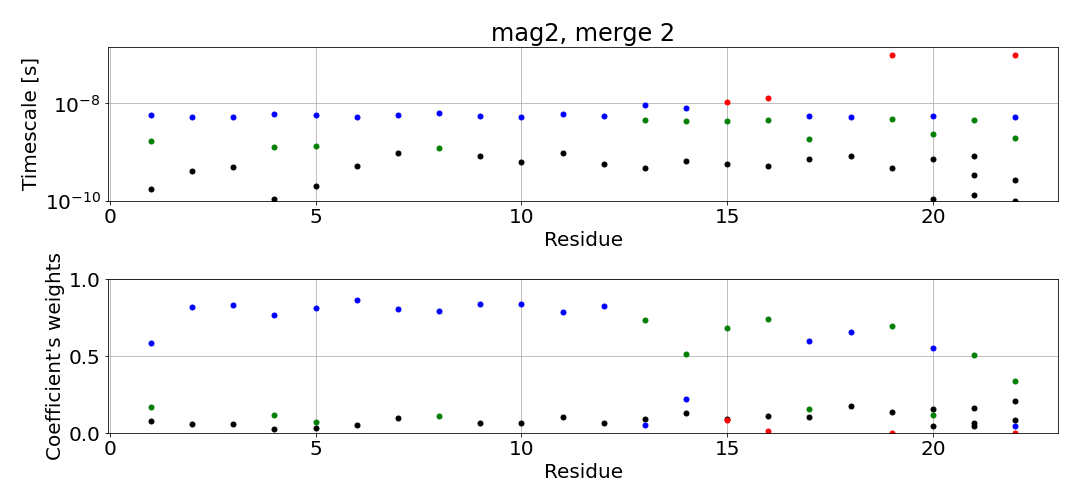
\includegraphics[width=0.5\textwidth]{mag2_2_slow.png}
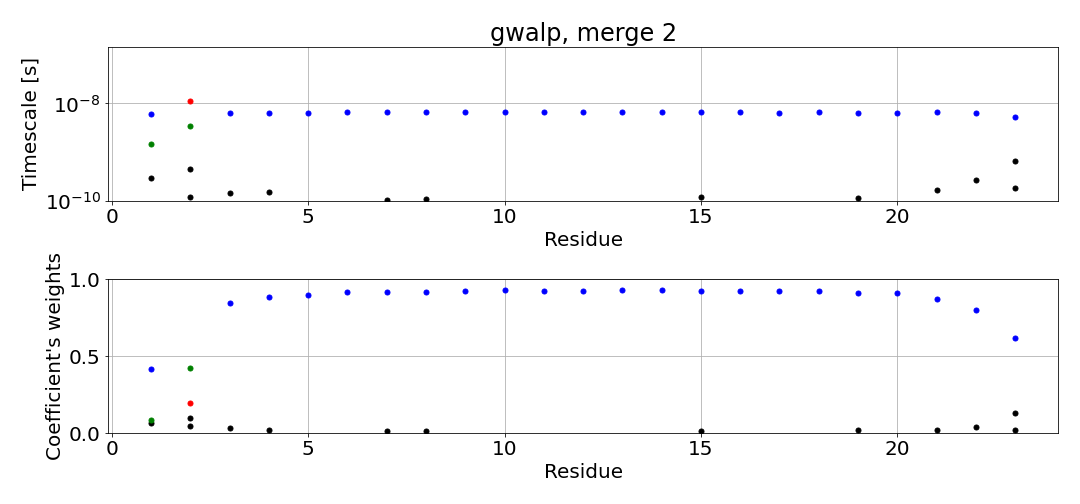
\includegraphics[width=0.5\textwidth]{gwalp_2_slow.png}
\end{figure}


\begin{figure}
\centering
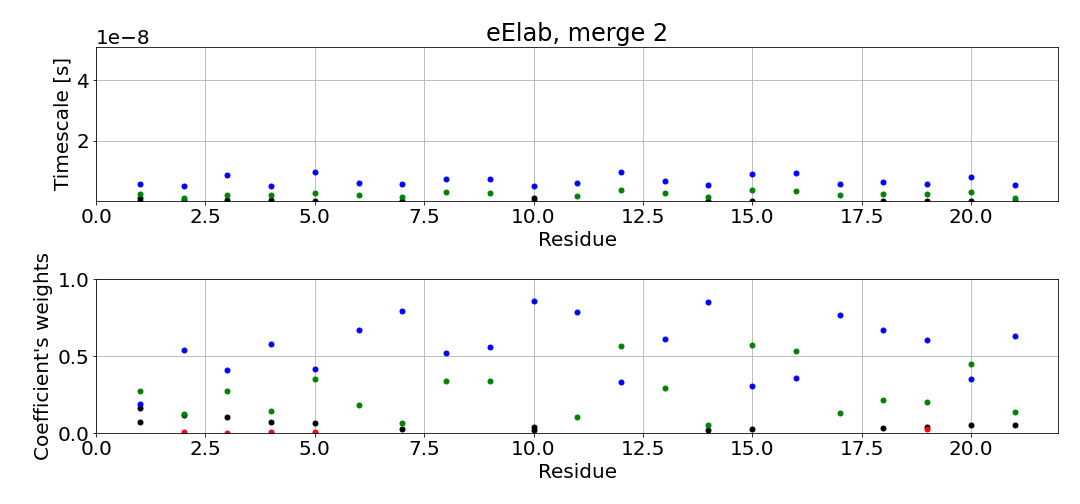
\includegraphics[width=0.5\textwidth]{eElab_2_slow_lin.png}
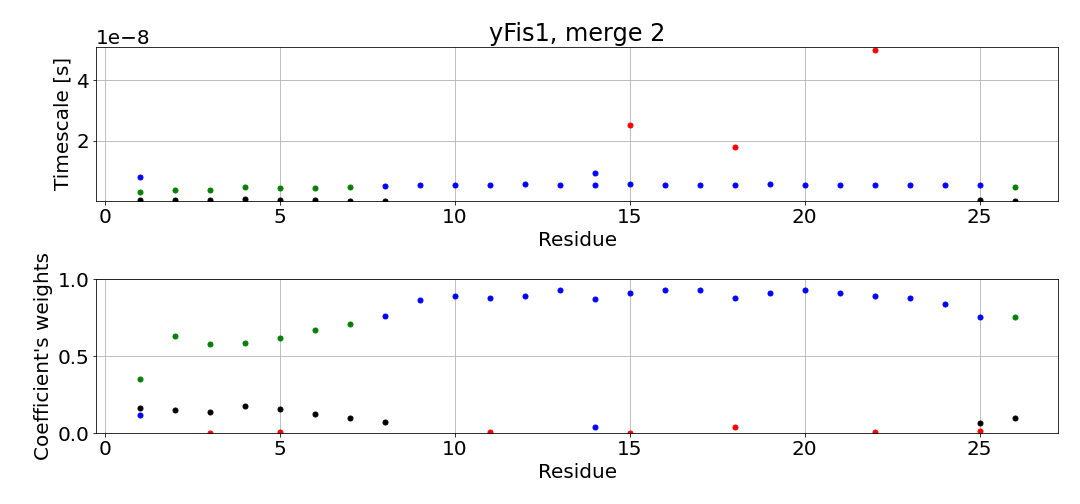
\includegraphics[width=0.5\textwidth]{yFis1_2_slow_lin.png}
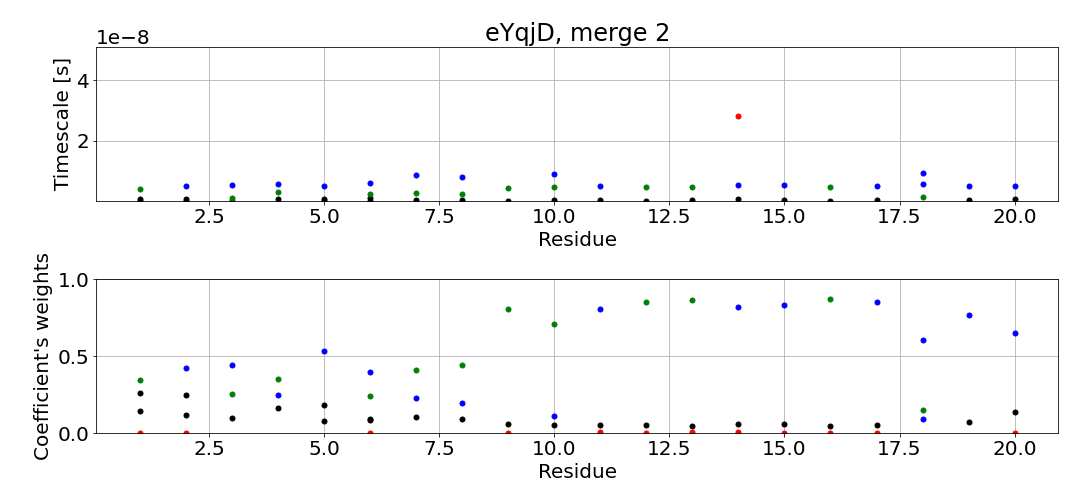
\includegraphics[width=0.5\textwidth]{eYqjD_2_slow_lin.png}
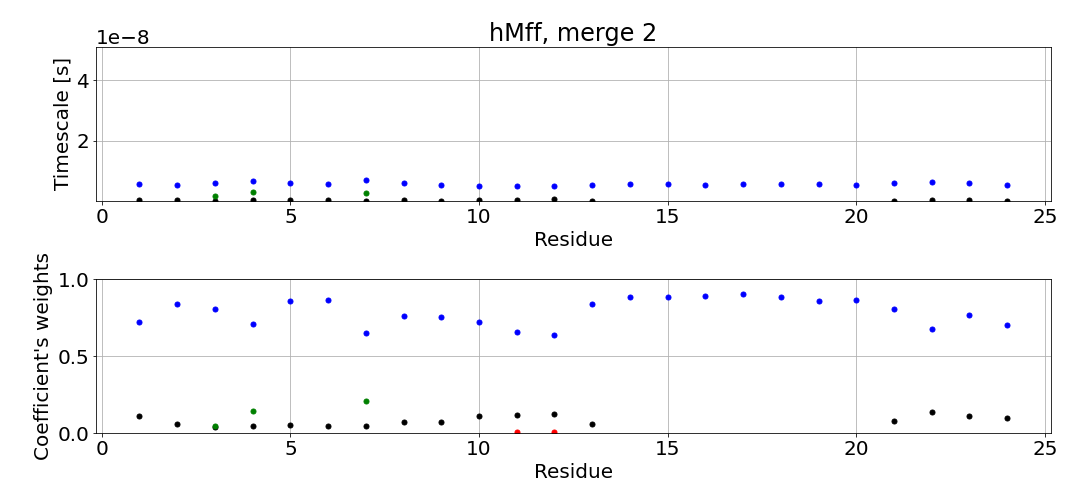
\includegraphics[width=0.5\textwidth]{hMff_2_slow_lin.png}
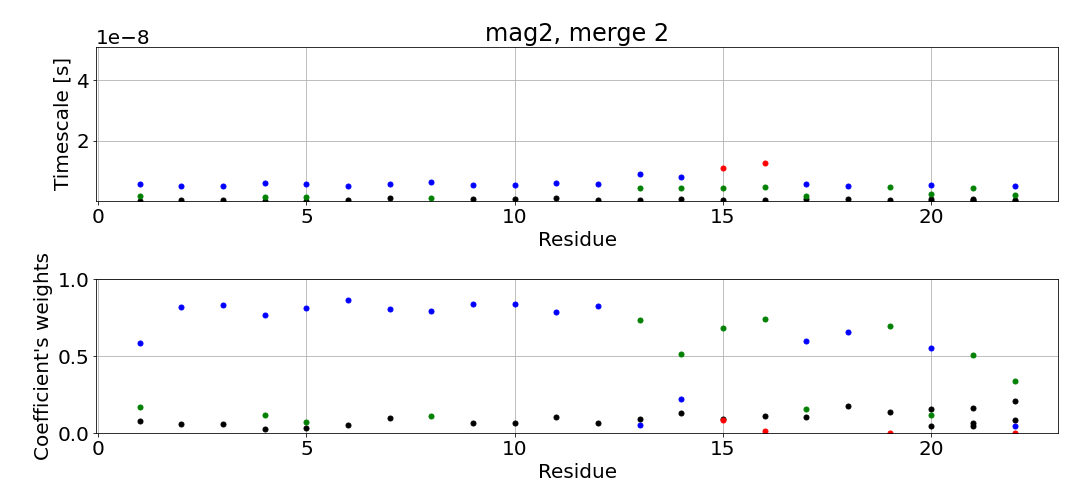
\includegraphics[width=0.5\textwidth]{mag2_2_slow_lin.png}
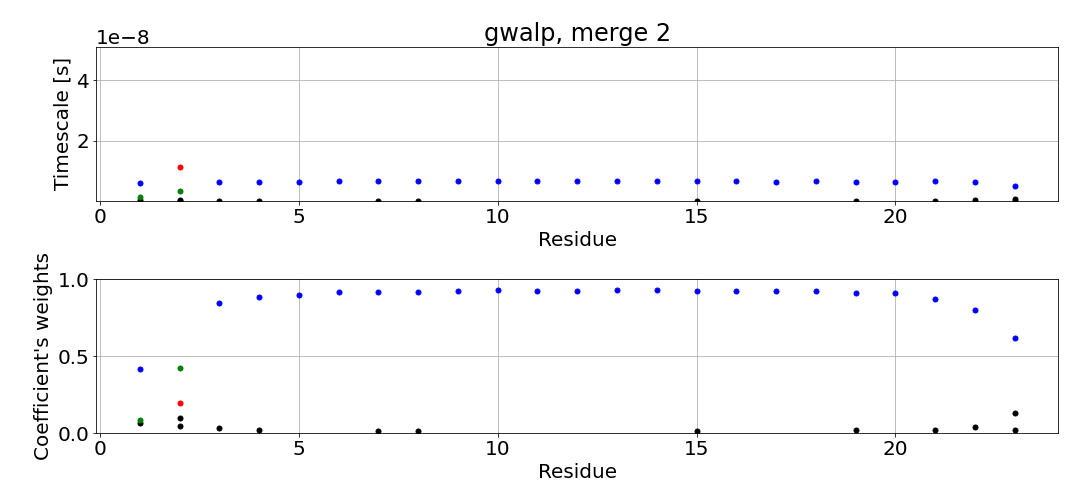
\includegraphics[width=0.5\textwidth]{gwalp_2_slow_lin.png}
\end{figure}

\end{document}